\documentclass{beamer}       % print frames
%\documentclass[notes=only]{beamer}   % only notes
%\documentclass{beamer}              % only frames
\newcounter{savedenum}
\newcommand*{\saveenum}{\setcounter{savedenum}{\theenumi}}
\newcommand*{\resume}{\setcounter{enumi}{\thesavedenum}}
\usepackage{multienum}
\usepackage[T1]{fontenc}
\usepackage{minted}
\usepackage{upquote}
\usepackage{tabularx}
\AtBeginDocument{%
\def\PYZsq{\textquotesingle}%
}
\usepackage[notocbib]{apacite}
    \renewcommand{\APACrefatitle}[2]{#1}
    \renewcommand{\APACrefbtitle}[2]{#1}
    \renewcommand{\APACrefbtitle}[2]{\Bem{#1}}
    \renewcommand{\APACrefaetitle}[2]{[#2]}
    \renewcommand{\APACrefbetitle}[2]{[#2]} 
\usepackage{textpos}
\usepackage{setspace}
\usefonttheme{serif}
%\usepackage{graphicx}
\usetheme{Boadilla}
\usepackage{hyperref}
\usepackage[UKenglish]{babel}
\usepackage{multicol}
\setcounter{tocdepth}{1} 
\usecolortheme{orchid}
\title[FEAST]{Shifting discourse-semantics of risk in US newspapers, 1987--2014}
\author[McDonald \& Zinn]{Daniel McDonald \and Jens Zinn~\\~\\\texttt{@interro\_gator}~\\~\\This slideshow is available at: \url{http://git.io/vBfbw}~\\~\\}

\date{\today}

\begin{document}

\addtobeamertemplate{frametitle}{}{%
\begin{textblock*}{100mm}(.775\textwidth,-.5cm)

\includegraphics[scale=.235]{../../images/unimelblong}
\end{textblock*}}

\frame{\titlepage}


\begin{frame}
    \frametitle{Overview}
    
    \begin{itemize}
    \item Context of the investigation: risk theory
    \item Data and research questions
    \item Linguistic approaches to risk
    \item Our methods and linguistic findings
    \item Sociological significance of the results
    \end{itemize}

    ~\\ This slideshow is available at: \url{http://git.io/vBfbw}

\end{frame}

\begin{frame}\frametitle{The project(s)}

I'm presenting work from closely related projects:

\begin{enumerate}
    \item Risk words in the NYT, 1963, 1987--2014
    \item Risk words in NYT health articles
    \item Risk words in six US newspapers, 1987--2014
\end{enumerate}

All investigations involve making longitudinally structured, parsed corpora and looking at how risk words behave.

\end{frame}

\begin{frame}
    \frametitle{Context: sociological risk theory}
    
    Risk as concept is sociologically important:

    \begin{itemize}
        \item New global risks \cite{beck_risk_1992}
        \item Calculative technologies \cite{dean_governmentality:_1999}
        \item Individualisation (from tradition to decision)
        \item Technologies of the Self \cite{dean_risk_1998}
        \item Risk-taking \cite{luhmann_risk:_1993}
    \end{itemize}

\end{frame}

\begin{frame}\frametitle{Context: risk as word}
\begin{itemize} 
    \item Risk can be nominal, verbal, adjectival, adverbial
    \item Risk as lexical item is increasingly frequent in print journalism (Zinn 2011)
    \item Risk as a lexical item in naturalistic text may behave contrary to expectations \cite{hamilton_meanings_2007}
    \item Meaning of risk moves toward \emph{threat\slash danger}
\end{itemize}
Risk as participant is more closely related to negative outcomes than risk as process:
\begin{itemize}
    \item \emph{They risked it all and won}
    \item \emph{Risks\slash rewards}
\end{itemize}
\end{frame}

\begin{frame}
    \frametitle{Context: new methodologies}

    New kinds of data and tools make it possible to empirically analyse risk language in new ways:
    
    \begin{itemize}
    \item Digitisation of newspapers means we have large, well-structured datasets
    \item Parsing makes it possible to search for lexical and grammatical features in tandem
    \item Programmatic approaches to social science research facilitate:
    \begin{itemize}
        \item Automation
        \item Reproducibility
        \item Transparency
        \item Ability to deploy methods on new data
        \item \emph{Objectivity?}
    \end{itemize}
    \end{itemize}
\end{frame}

\begin{frame}
    \frametitle{The data}

    \begin{enumerate}
        \item \emph{NYT Annotated Corpus}: 1.8 million articles, 1987--2007 \cite{sandhaus_new_2008}
        \item \emph{ProQuest Newsstand} for NYT 2007--2014
        \item \emph{ProQuest Newsstand} for five other newspapers, 1987--2014
        \begin{enumerate}
            \item \emph{Washington Post}
            \item \emph{Tampa Bay Times}
            \item \emph{USA Today}
            \item \emph{Chicago Tribune}
            \item \emph{Wall Street Journal}
        \end{enumerate}
        \item 54,288,152 words
        \item 1,031,208 risk words
        \item 43GB when parsed
    \end{enumerate}
\end{frame}

\begin{frame}
    \frametitle{Increasing frequency of \emph{risk} lemma}
    \centering
    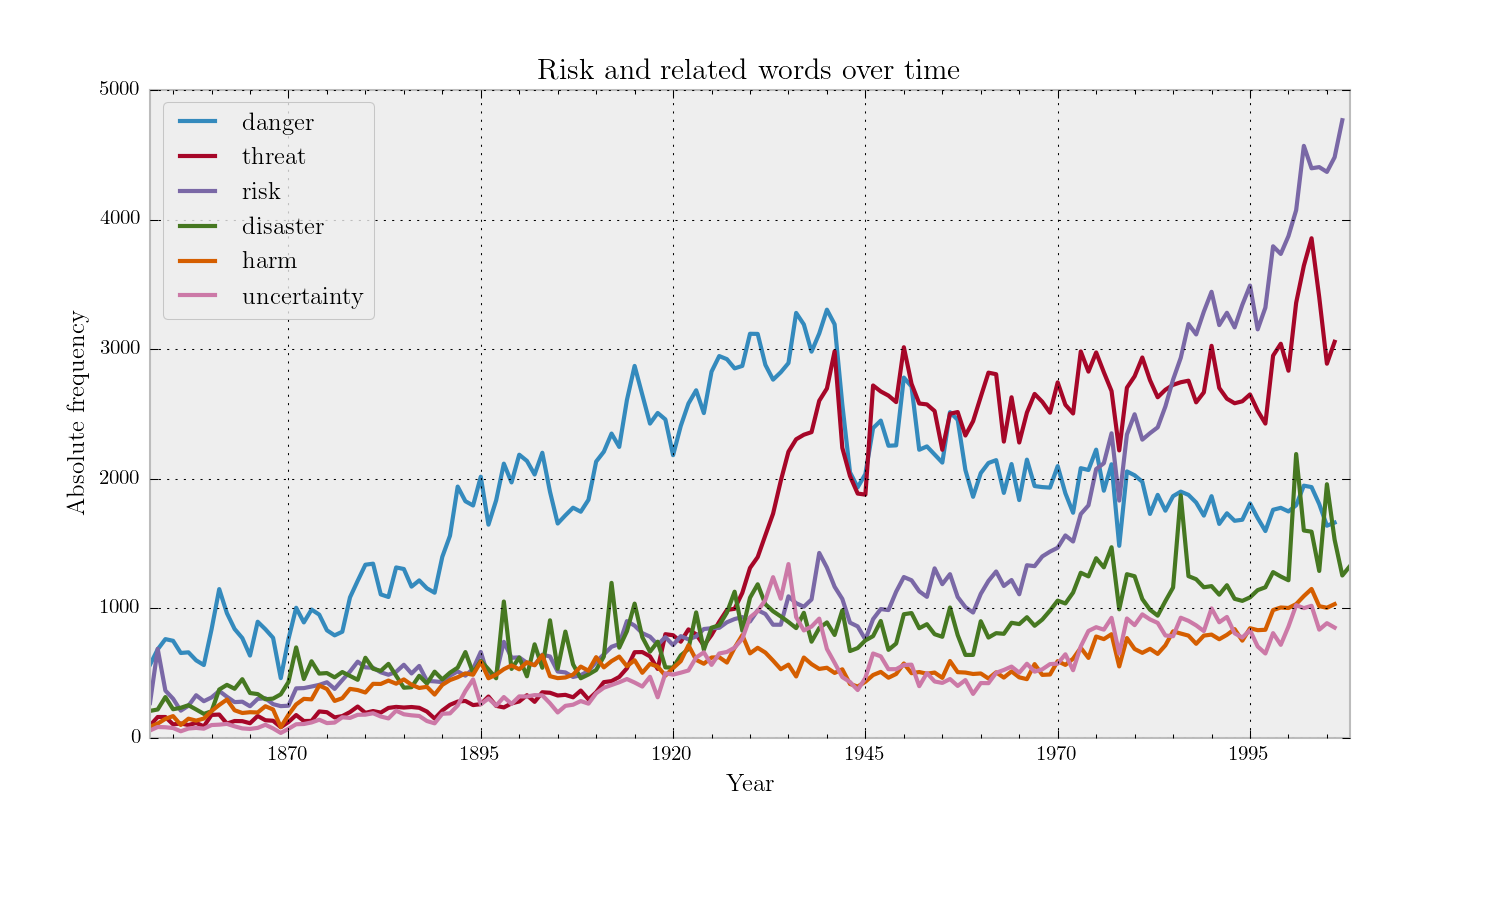
\includegraphics[width=1\textwidth]{../../images/risk_related_june_colour}
\end{frame}

\begin{frame}
    \frametitle{Research questions}

    We span the sociological, linguistic and computational:

    \begin{enumerate}
        \item How does the institutionalisation of new societal practices manifest linguistically in the change of risk discourses and the use of risk language?
        \item How do risk words behave longitudinally at the lexicogrammatical and discourse-semantic strata?
        \item What kinds of tools or methods are needed for this kind of (digital humanities) research?
    \end{enumerate}
\end{frame}

\begin{frame}
    \frametitle{Linguistics: frame semantic approach}

    Frame semantics: risk as a cognitive schema \cite{fillmore_toward_1992}

\begin{itemize}
    \item Conceptualises risk mostly as experiential Process\slash Event
    \begin{itemize}
        \item \emph{What kind of participants and circumstances occur when risk is the Process?}
    \end{itemize}
    \item Problem: risk often takes less prominent experiential roles
    \begin{itemize}
        \item Is the risk frame actually invoked when the word is used?
        \item Example:
    \end{itemize}
    \end{itemize}

    ~\\
    \footnotesize
    \begin{quote}
    \noindent
    \texttt{Mr. Tepfer noted that Mr. Douglas, who was in the neighborhood when the body was found and was interviewed by the police at the time, `preyed on \textbf{at-risk women}, on prostitutes, and he engaged in sex and strangled them to death.' }
    \end{quote}

\end{frame}

\begin{frame}
    \frametitle{The risk frame}
    \centering
    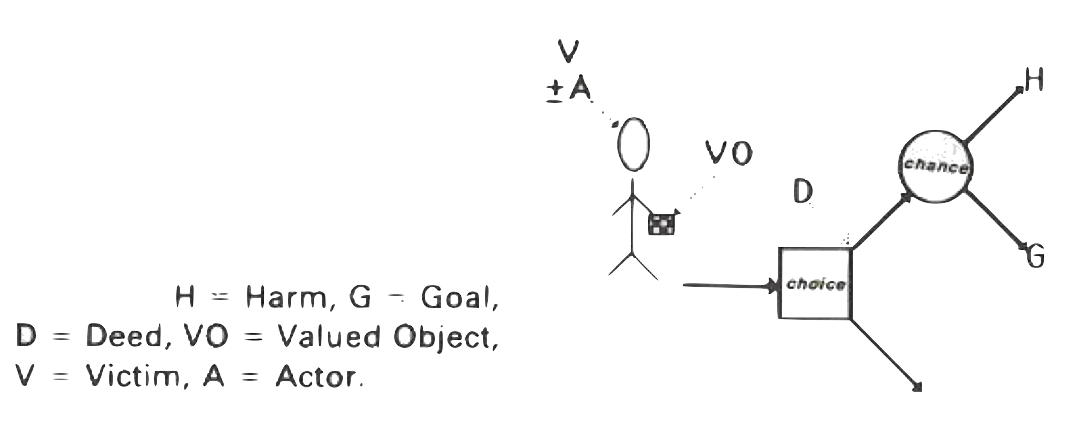
\includegraphics[width=0.90\textwidth]{../../images/riskframe.png}
\end{frame}


\begin{frame}
    \frametitle{Corpus linguistic approach}

    Corpus linguistics: risk as token \cite{hamilton_meanings_2007}

    \begin{itemize}
    \item Topics and text-types in which risk tokens appear
    \item Collocates of risk tokens
    \item Risk appears a lot in discussions of health
    \item Use of risk words is different to invented examples
    \end{itemize}

    Shortcomings:

    \begin{itemize}
        \item Smaller corpus size, heterogeneity of samples
        \item No parsing, lemmatisation
        \item No systematic connection of lexicogrammatical patterns to discourse\slash meaning
    \end{itemize}

\end{frame}

\begin{frame}
    \frametitle{Our methods}
    
    \begin{itemize}
    \item Get all paragraphs containing \texttt{\textbackslash brisk} in all 1987--mid 2014 articles
    \item Annotate\slash parse the data with full \emph{Stanford CoreNLP} suite with embarrassingly parallel HPC
    \item Develop \texttt{corpkit}, a toolkit for searching the corpus and communicating results
    \item Interrogate the corpus according to notions from systemic functional grammar
    \item Connect to sociological theory
    \end{itemize}
\end{frame}

\begin{frame}
\frametitle{SFL: the basics}
\begin{itemize}
\item \emph{Systemic}: lexis as delicate grammar
\item \emph{Functional}: focus on language as a tool for the performance of functions
\begin{enumerate}
    \item Interpersonal: negotiating relationships
    \item \textbf{Experiential: representing the world}
    \item Textual: reflexive organisation into meaningful sequences
\end{enumerate}
\end{itemize}
\end{frame}

\begin{frame}
    \frametitle{Overview of SFL}
    \centering
    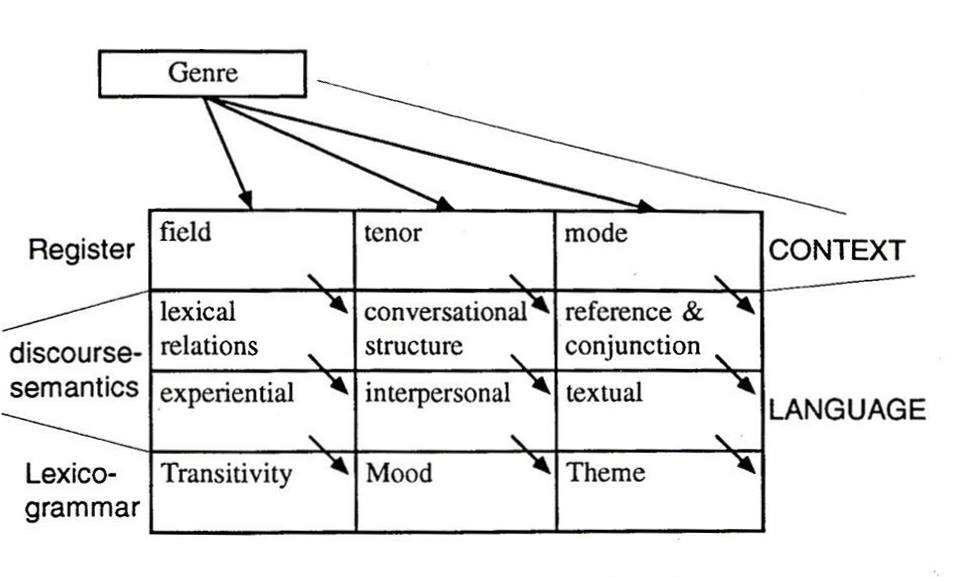
\includegraphics[width=0.90\textwidth]{../../images/egginsfixed.jpg}
\end{frame}

\begin{frame}\frametitle{Transitivity system}
\begin{itemize}
    \item Focus on the clause as a unit of analysis
    \item Centre on the \emph{process} (i.e. rightmost verb in VP)
    \item Processes \emph{select} participants (i.e. arguments of the verb)
    \item PPs and RBs are typically \emph{circumstances}
\end{itemize}
\end{frame}

\begin{frame}\frametitle{SF transitivity analysis}

~\\
~\\
\small
\begin{tabularx}{0.99\textwidth}{|l|l|X|X|X|}
\hline
\emph{But}     & \emph{the bang of the gavel}             & \emph{can hold}          & \emph{risk} & \emph{for novices}          \\ \hline
~ & Participant: & Process: & Participant: & Circumstance:  \\
~ & Carrier & Relational \mbox{attributive} & Attribute &  Extent \\ \hline
\end{tabularx}
\end{frame}

\begin{frame}
    \frametitle{Constituency grammar}
    \centering
    \includegraphics[width=0.67\textwidth]{../../images/const-grammar}
\end{frame}

\begin{frame}
    \frametitle{Dependency grammar}
    \centering
    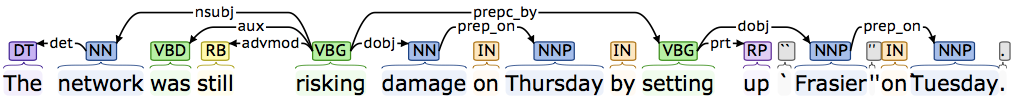
\includegraphics[width=0.99\textwidth]{../../images/depparse}
\end{frame}

\begin{frame}\frametitle{The controversial question}

The question: \emph{Can we get systemic functional information from constituency and dependency parses?}

~\\~\\~\\~\\

The answer: \emph{Yep, quite a lot.}
\end{frame}

\begin{frame}\frametitle{Developing tools}
How to investigate this huge dataset, and make the investigation transparent\slash reproducible?

\begin{itemize}
    \item \texttt{corpkit}: a Python module designed for parsed and structured corpora
    \begin{itemize}
        \item \texttt{interrogator()}: search for lexicogrammatical phenomena in each subcorpus, tally results, output Pandas objects
        \item \texttt{editor()}: edit results, calculate keyness, linear regression 
        \item \texttt{plotter()}: visualise via \emph{matplotlib} 
        \item \texttt{conc()}: concordance via parses 
    \end{itemize}
    \item Scriptable, multiprocessing, handles arbitrary data, open-source
    \item Systemic-functionally aware
    \item More recently, a GUI, aimed at corpus linguists
\end{itemize}
\end{frame}

\begin{frame}
    \frametitle{\texttt{corpkit} GUI: interrogating}
    \centering
    \includegraphics[width=0.95\textwidth]{../../images/interrogate}
\end{frame}

\begin{frame}
    \frametitle{\texttt{corpkit}: concordancer}
    \centering
    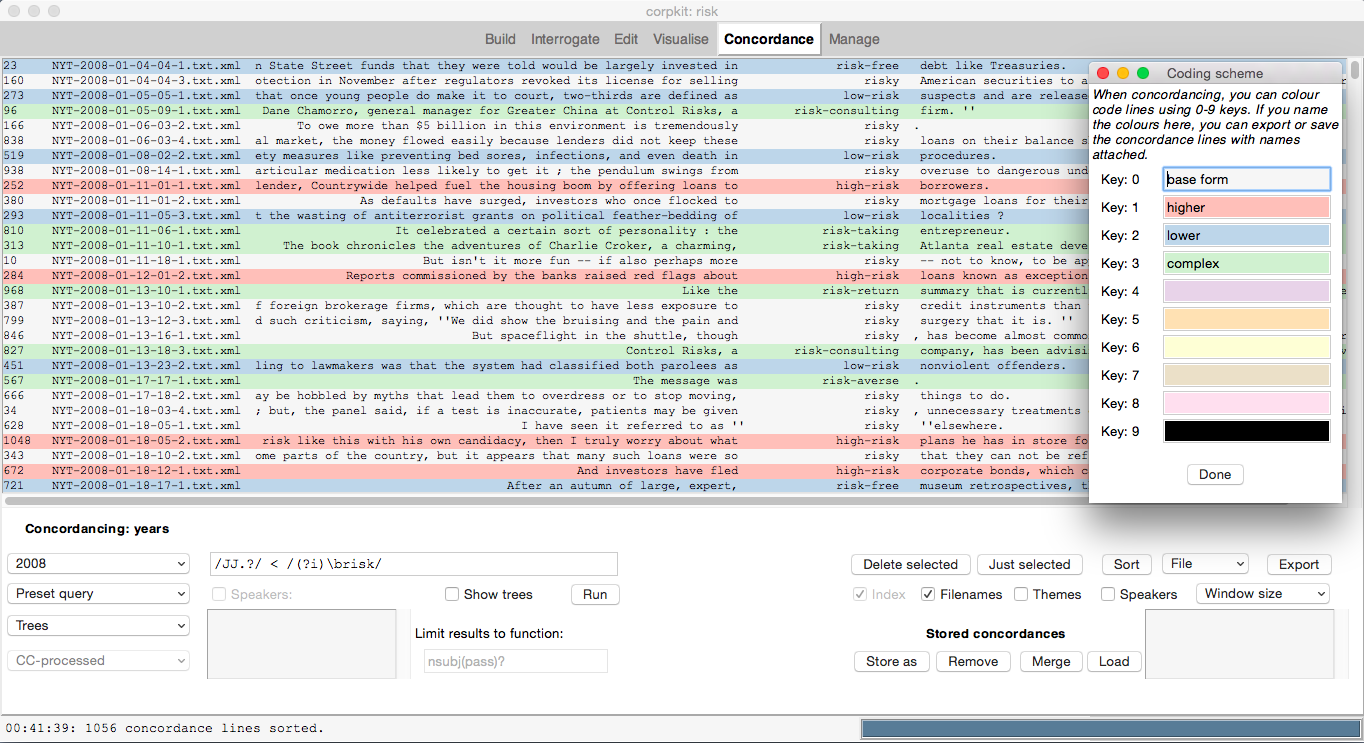
\includegraphics[width=0.95\textwidth]{../../images/conc2}
\end{frame}

\begin{frame}
    \frametitle{\texttt{corpkit}: plotting}
    \centering
    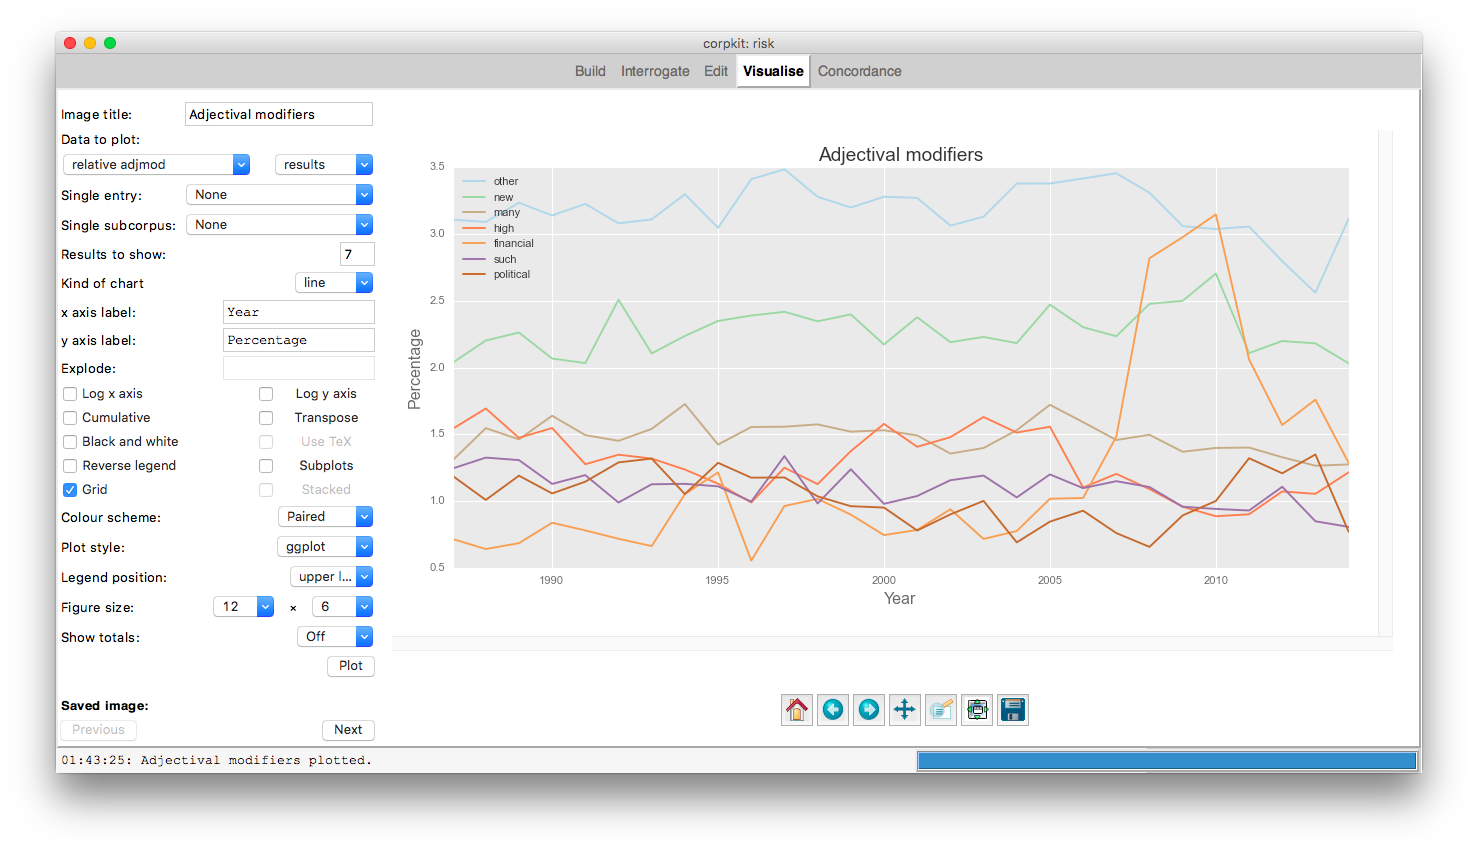
\includegraphics[width=0.95\textwidth]{../../images/plott}
\end{frame}

\begin{frame}[fragile]
\frametitle{\texttt{corpkit}: example code}

\begin{minted}[fontsize=\normalsize,linenos=true]{python}
# import module and set data path
>>> from corpkit import *
>>> corpus = 'data/NYT-parsed'

# get pos of risk words, show word class
>>> res = interrogator(corpus, 'words', r'\brisk', 
...    show = ['p'], lemmatise = True)

# get relative frequency
>>> rel = editor(res.results, '%', res.totals, keep_top = 4)

# visualise
>>> plotter('Word class of risk words', rel.results, 
...    kind = 'area', style = 'seaborn-talk')
\end{minted}
\end{frame}

\begin{frame}
    \frametitle{Example output}
    \centering
    \includegraphics[width=0.90\textwidth]{../../images/pos_sb}
\end{frame}

\begin{frame}
    \frametitle{Nominalisation of risk in the NYT}
    \centering
    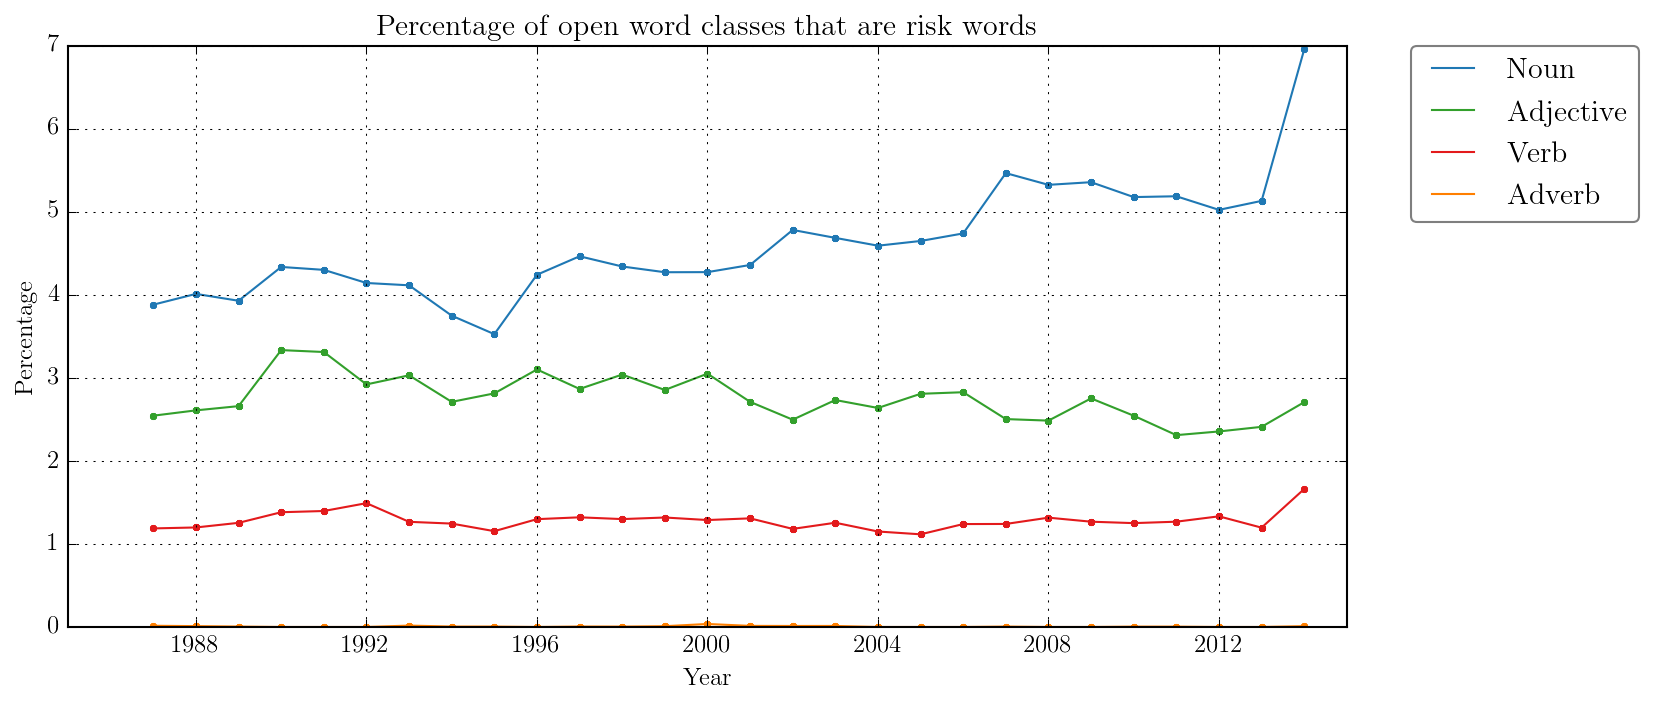
\includegraphics[width=0.99\textwidth]{../../images/percentage-of-open-word-classes-that-are-risk-words}
\end{frame}

\begin{frame}
    \frametitle{Experiential roles of risk words}
    \centering
    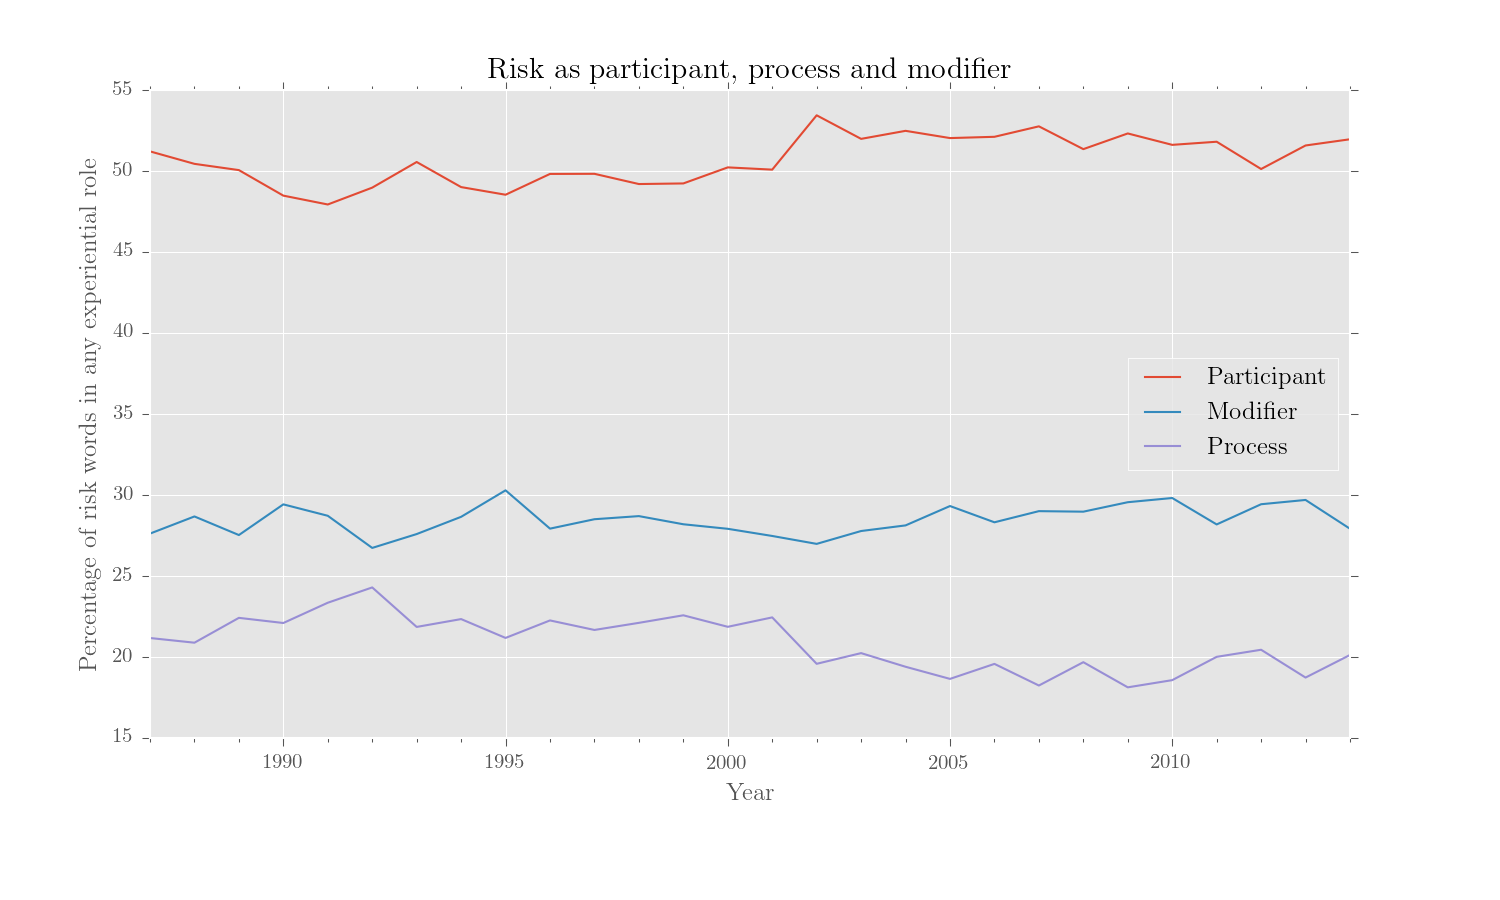
\includegraphics[width=0.99\textwidth]{../../images/ppm_final_colour}

    \noindent \emph{They risked their life} $\rightarrow$ \emph{It was a risk}
\end{frame}

\begin{frame}
    \frametitle{Risk as modifier}
    \centering
    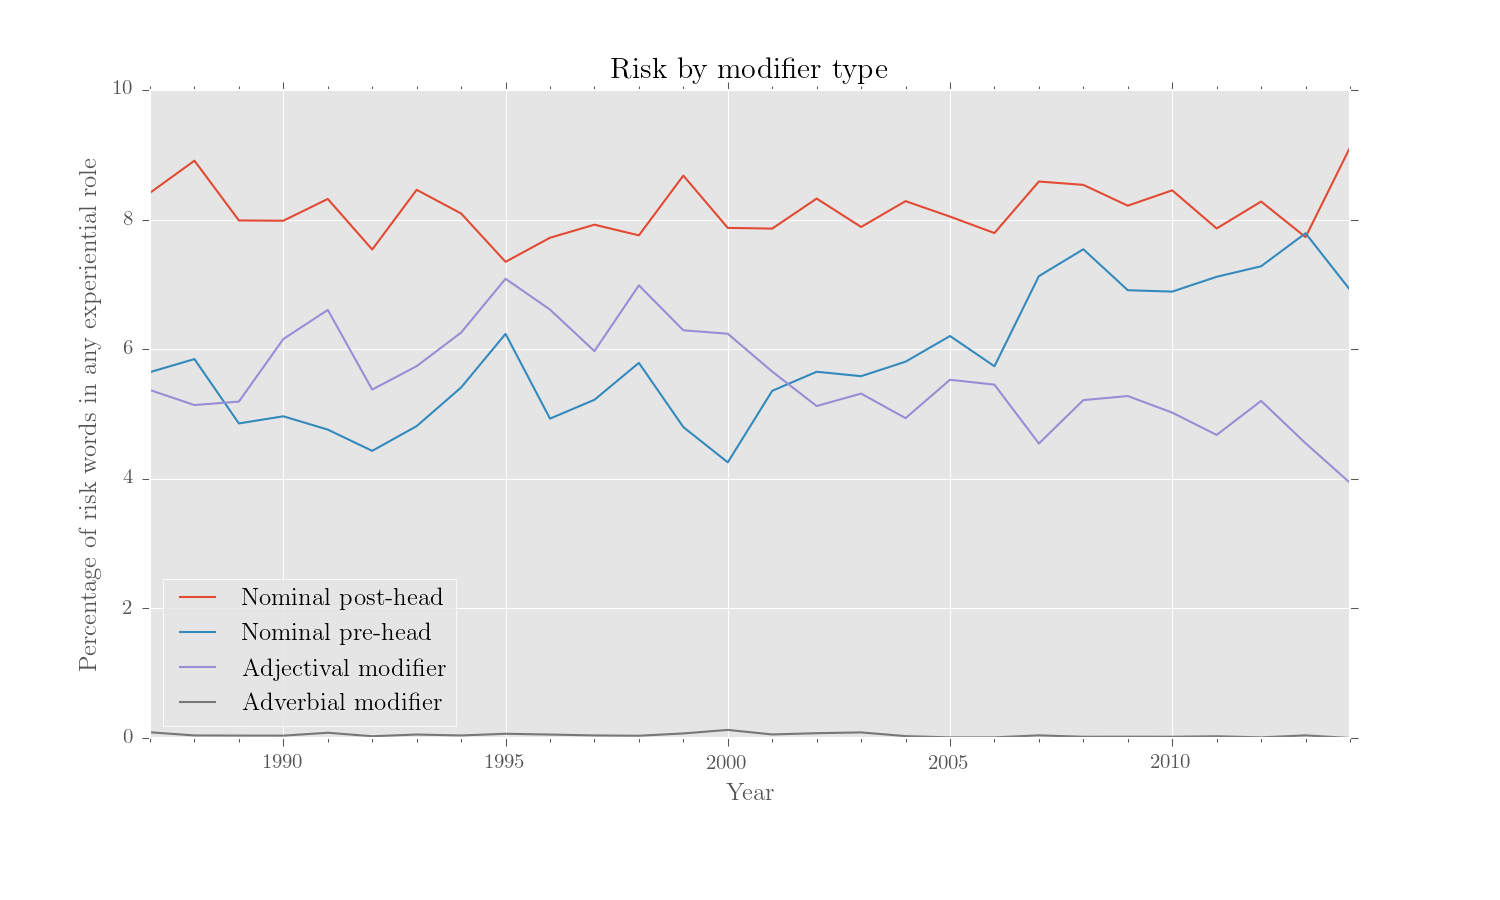
\includegraphics[width=0.99\textwidth]{../../images/risk_by_mod_type_colour}

    \noindent \emph{Risky decision} $\rightarrow$ \emph{risk assessment}
\end{frame}

\begin{frame}
    \frametitle{Risk and power}
    \centering
    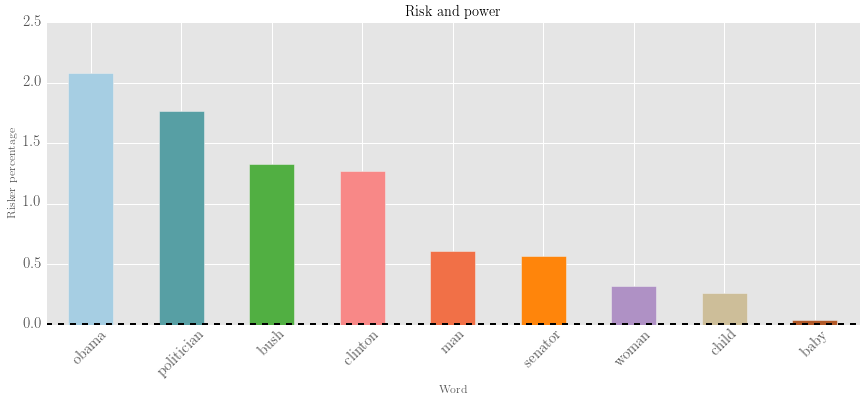
\includegraphics[width=0.99\textwidth]{../../images/risk-and-power-2}

    $\rightarrow$ Powerful and influential people \emph{do} risking

\end{frame}

\begin{frame}
    \frametitle{Distance of risk word from \emph{root}}
    \centering
    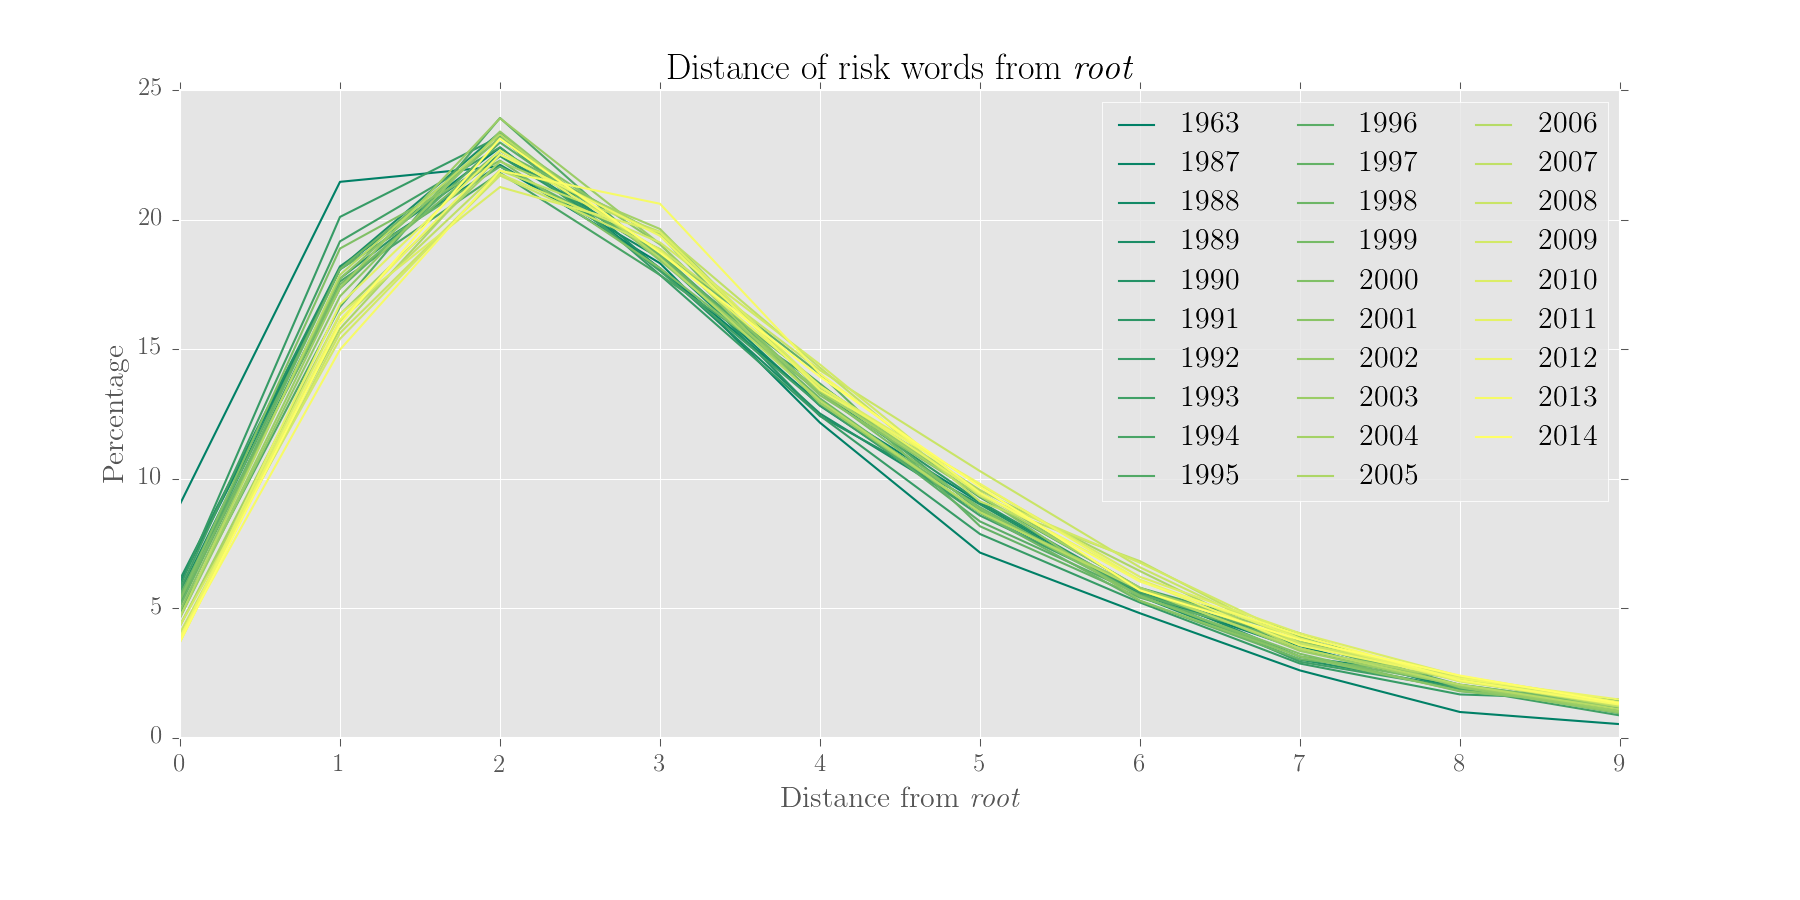
\includegraphics[width=1\textwidth]{../../images/distance-of-risk-words-from-root}

    $\rightarrow$ looked promising, but seems to be a general phenomenon.
\end{frame}

\begin{frame}
    \frametitle{Mood role of risk words (NYT)}
    \centering
    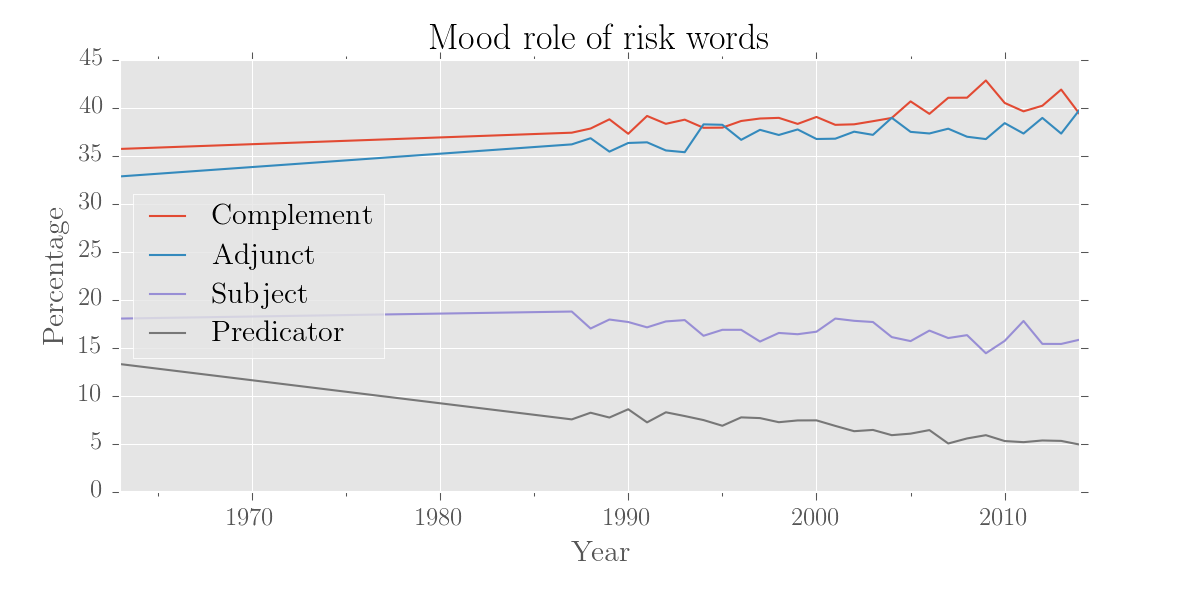
\includegraphics[width=1\textwidth]{../../images/mood-role-of-risk-words}

    Arguable $\rightarrow$ inarguable
\end{frame}


\begin{frame}
    \frametitle{First investigation: key findings}
    
    \begin{itemize}
    \item Nominalisation and \emph{participantification}: synonymy of risk and negative outcome
    \begin{itemize}
        \item risking harm $\rightarrow$ risk assessment
        \item Meaning of risk expanding beyond the \emph{risk frame}
    \end{itemize}
    \item Risk words becoming more implicit
    \begin{itemize}
        \item Routinisation of the management of risk
        \item Risk as increasingly present, but decreasingly debated
    \end{itemize}
    \item More everyday exposure to risk, but less risking
    \item Neoliberal conceptualisations of agency: institutional expectation to take risk, absolution of responsibility for institutions themselves
    \end{itemize}
\end{frame}

\begin{frame}\frametitle{Health risk}

\begin{itemize}
\item As earlier studies have shown, risk words often occur in health domains.
\item The NYT Annotated Corpus had some manually added topic tags
\item We created a subcorpus of health articles
\end{itemize}
\end{frame}

\begin{frame}
    \frametitle{Decreasing participants in health discourse}
    \centering
    \includegraphics[width=0.99\textwidth]{../../images/decline-of-health-institution-risks-in-the-nyt-1987-2014}
\end{frame}

\begin{frame}
    \frametitle{Increasing participants in health discourse}
    \centering
    \includegraphics[width=0.99\textwidth]{../../images/part_health_inc_final_colour}
\end{frame}

\begin{frame}\frametitle{Six newspapers}
\begin{itemize}
\item We've only just started interrogating the six newspaper corpus
\item First, we'd like to check if the NYT findings are generalisable to other publications.
\item Then, understanding the reason for differences and similarities would be nice
\item Would love help on dealing with the complexity of the data structure!
\end{itemize}
\end{frame}

\begin{frame}\frametitle{\emph{To take risk}}
    \centering
    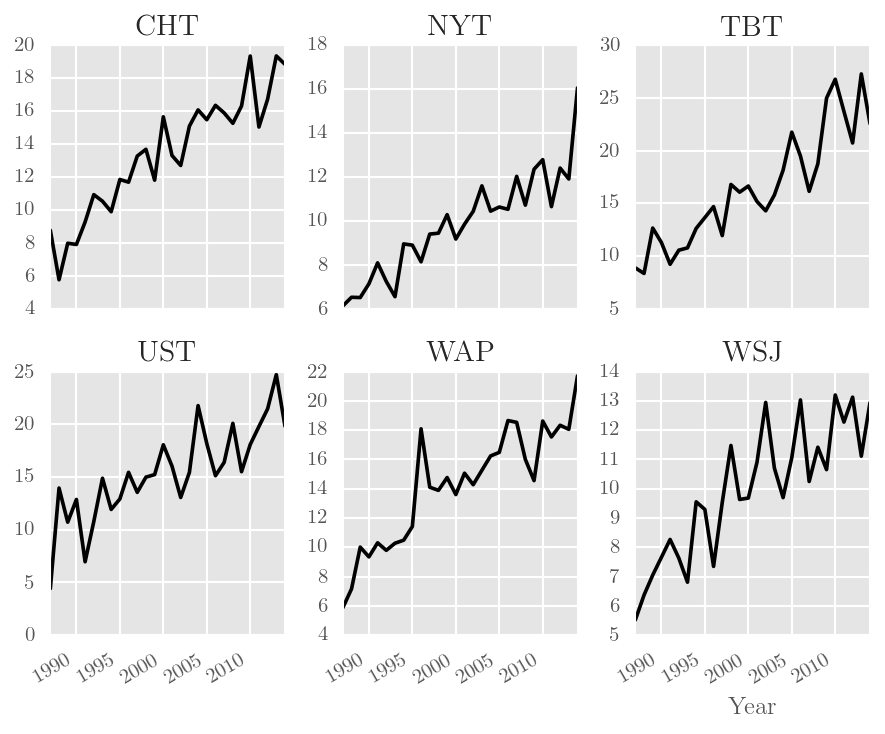
\includegraphics[width=.9\textwidth]{../../images/to-put-at-risk}
\end{frame}

\begin{frame}\frametitle{\emph{To put at risk}}
    \centering
    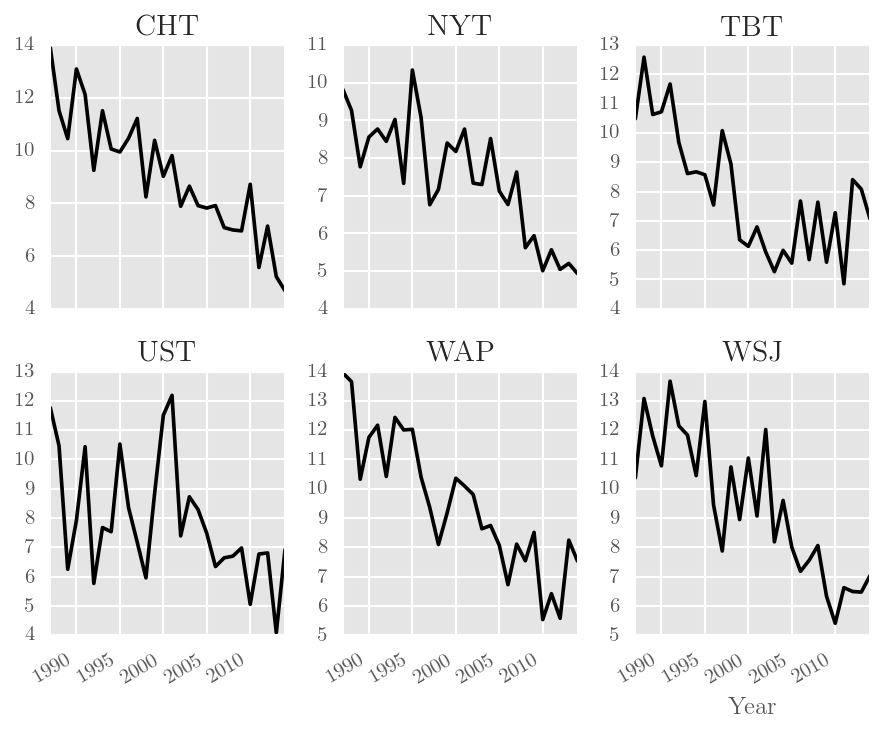
\includegraphics[width=.9\textwidth]{../../images/to-run-risk}
\end{frame}

\begin{frame}\frametitle{\emph{Risk processes}}
    \centering
    \includegraphics[width=1\textwidth]{../../images/longitudinal-behaviour-of-risk-processes-in-us-print-media}
\end{frame}

\begin{frame}\frametitle{Less risking}
    \centering
    \includegraphics[width=1\textwidth]{../../images/percentage-of-noun-lemmata-in-the-risker-position}
\end{frame}

\begin{frame}\frametitle{Risk and power across publications}
    \centering
    \includegraphics[width=1\textwidth]{../../images/rp6}
\end{frame}

\begin{frame}
    \frametitle{Mood role of risk words}
    \centering
    \includegraphics[width=1\textwidth]{../../images/moodrole-6}
    Arguable $\rightarrow$ inarguable
\end{frame}


\begin{frame}\frametitle{Preliminary findings}
\begin{itemize}
    \item Many phenomena generalisable
    \item Some newspaper specific constructions: \emph{risk appetite} in the WSJ
    \item Fewer grammatical riskers, but risk characterising more participants and processes
    \item Hints of influence of newspaper's politicIan position
\end{itemize}
\end{frame}

\begin{frame}
    \frametitle{Discussion: using SFL}
    \begin{itemize}
    \item SFL proves a useful means of dividing up and investigating the behaviour of a given word
    \item Systemic categories are \emph{sometimes} more telling than formal\slash constituency\slash dependency labels
    \item Though theoretical orientations are different, much of the grammar (esp. at group\slash phrase levels) are actually very similar
    \end{itemize}
\end{frame}

\begin{frame}\frametitle{Limitations}

\begin{itemize}
    \item This is a study of risk words, not risk
    \item Congruent realisations are analysed at the expense of the incongruent
    \item Little concordancing, close reading of individual texts
    \item Parser accuracy
    \item Lack of reference corpus to compare related words\slash general language
\end{itemize}
    
\end{frame}

\begin{frame}
    \frametitle{It's all open source}
    Data and tools are available for reuse:
    \begin{itemize}
    \item \url{https://www.github.com/interrogator/risk}
    \item \url{https://www.github.com/interrogator/corpkit}
    \end{itemize}
    Findings are presented dynamically in an Jupyter Notebook: 
    \begin{itemize}
    \item NYT: \url{http://git.io/vIM2W}
    \item All: \url{http://git.io/vBTHI}
    \end{itemize}
    Project report:
    \begin{itemize}
        \item \url{http://git.io/vZ7yh}
    \end{itemize}
    This slideshow:
    \begin{itemize}
    \item \url{http://git.io/vBfbw}
    \end{itemize}
\end{frame}

    \begin{frame}[t,allowframebreaks]
    \frametitle{References}
    \bibliographystyle{apacite}
    \bibliography{../report/references/references}
    \end{frame}
    
    \end{document}